\section{Результат выполнения программы}

Скриншот главной страницы приложения (рис. \ref{fig:fig-home})

\begin{figure}[H]
    \centering
    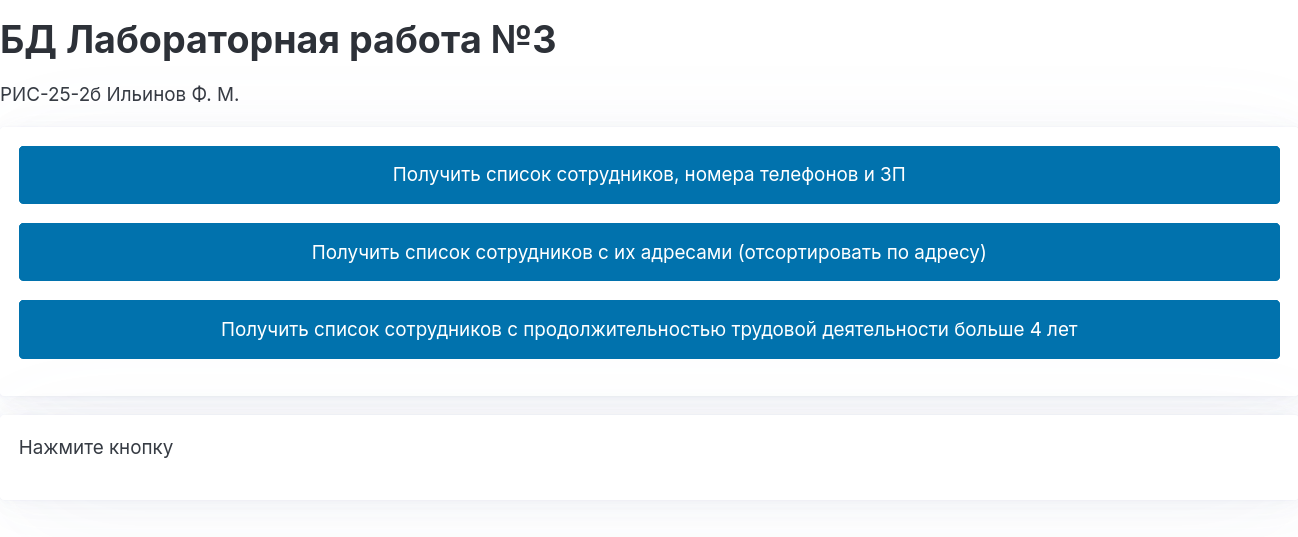
\includegraphics[width=1\textwidth]{img_home}
    \caption{Главная страница}
    \label{fig:fig-home}
\end{figure}

Скриншоты выполнения первого запроса: список сотрудников с номерами телефонов и заработной платой 
в браузере (рис. \ref{fig:fig-query1-browser}) и в просмотрщике баз данных (рис. \ref{fig:fig-query1-sql}).

\begin{figure}[H]
    \centering
    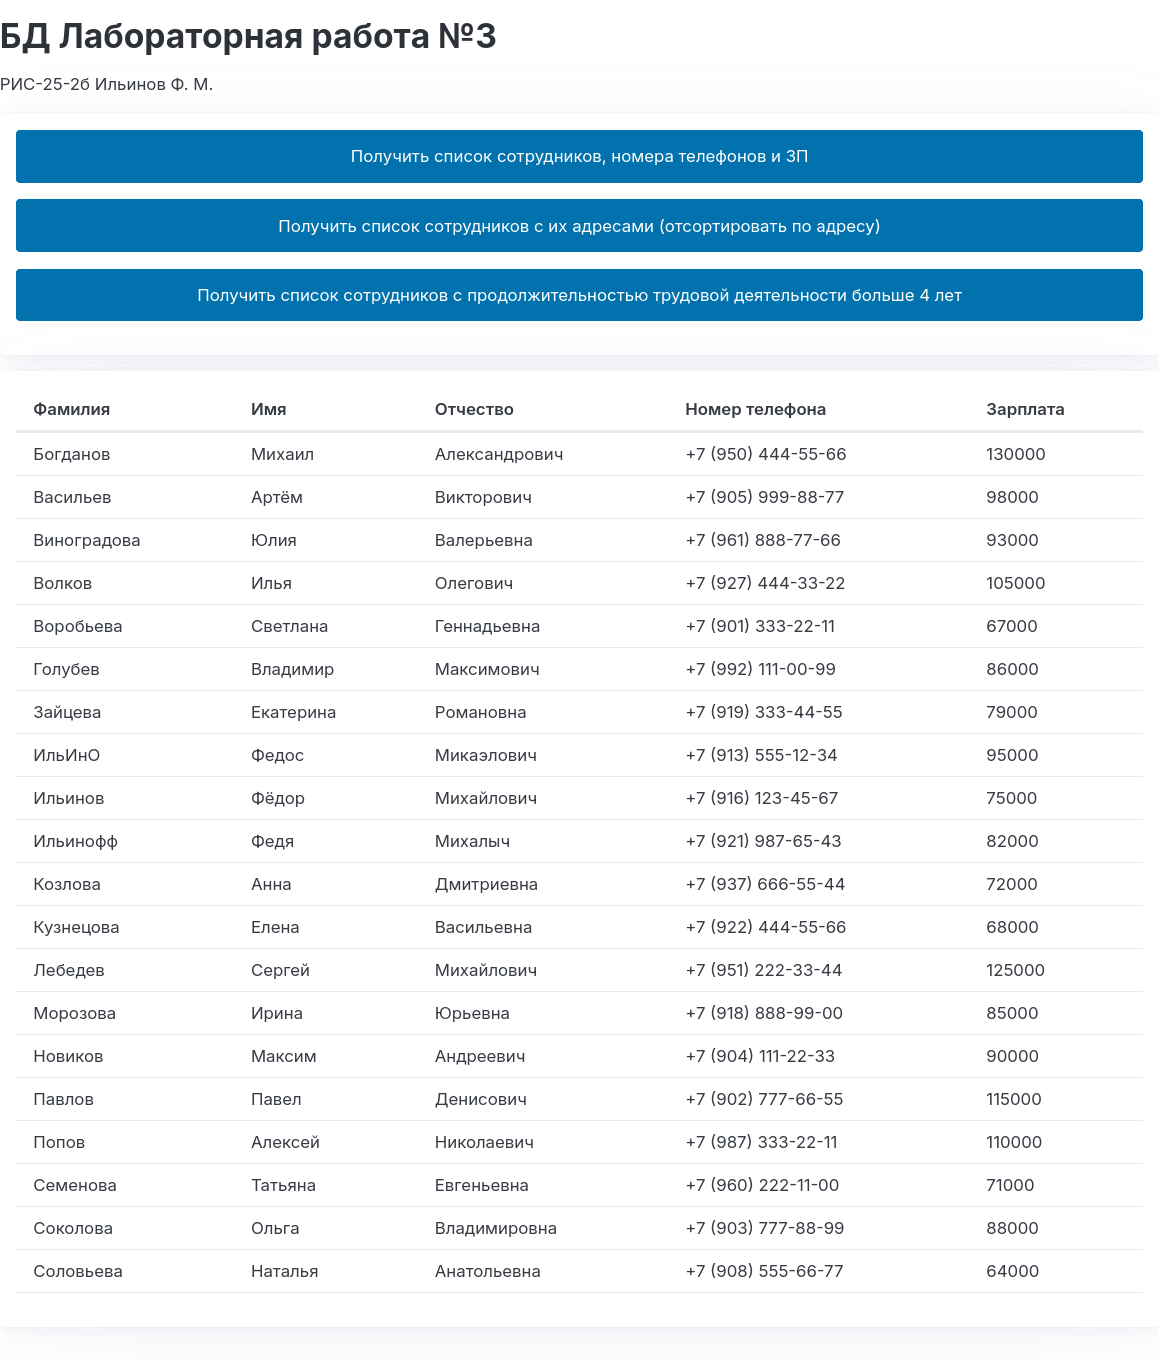
\includegraphics[width=1\textwidth]{img_query1_browser}
    \caption{Результаты выполнения первого запроса в браузере}
    \label{fig:fig-query1-browser}
\end{figure}

\begin{figure}[H]
    \centering
    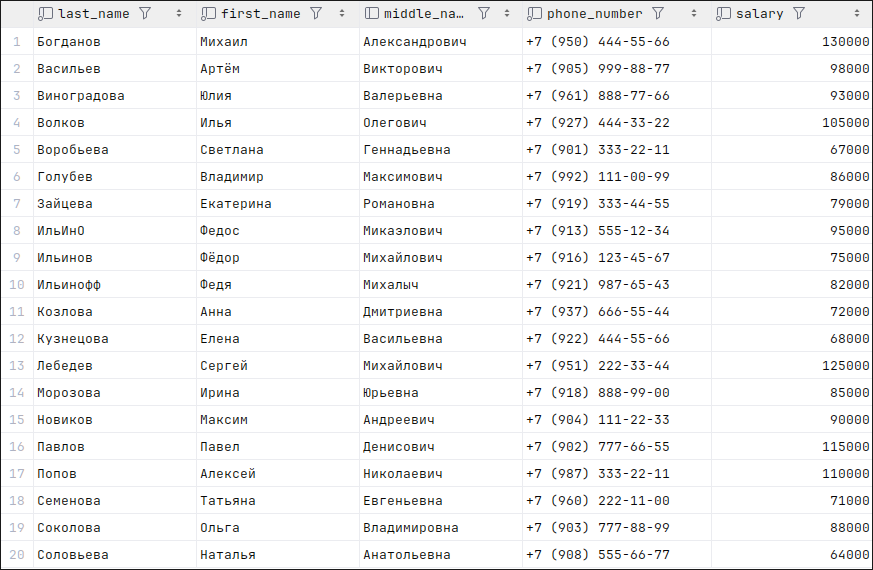
\includegraphics[width=1\textwidth]{img_query1_sql}
    \caption{Результаты выполнения первого запроса в просмотрщике баз данных}
    \label{fig:fig-query1-sql}
\end{figure}


Скриншот выполнения второго запроса: список сотрудников, отсортированный по адресу
в браузере (рис. \ref{fig:fig-query2-browser}) и в просмотрщике баз данных (рис. \ref{fig:fig-query2-sql}).

\begin{figure}[H]
    \centering
    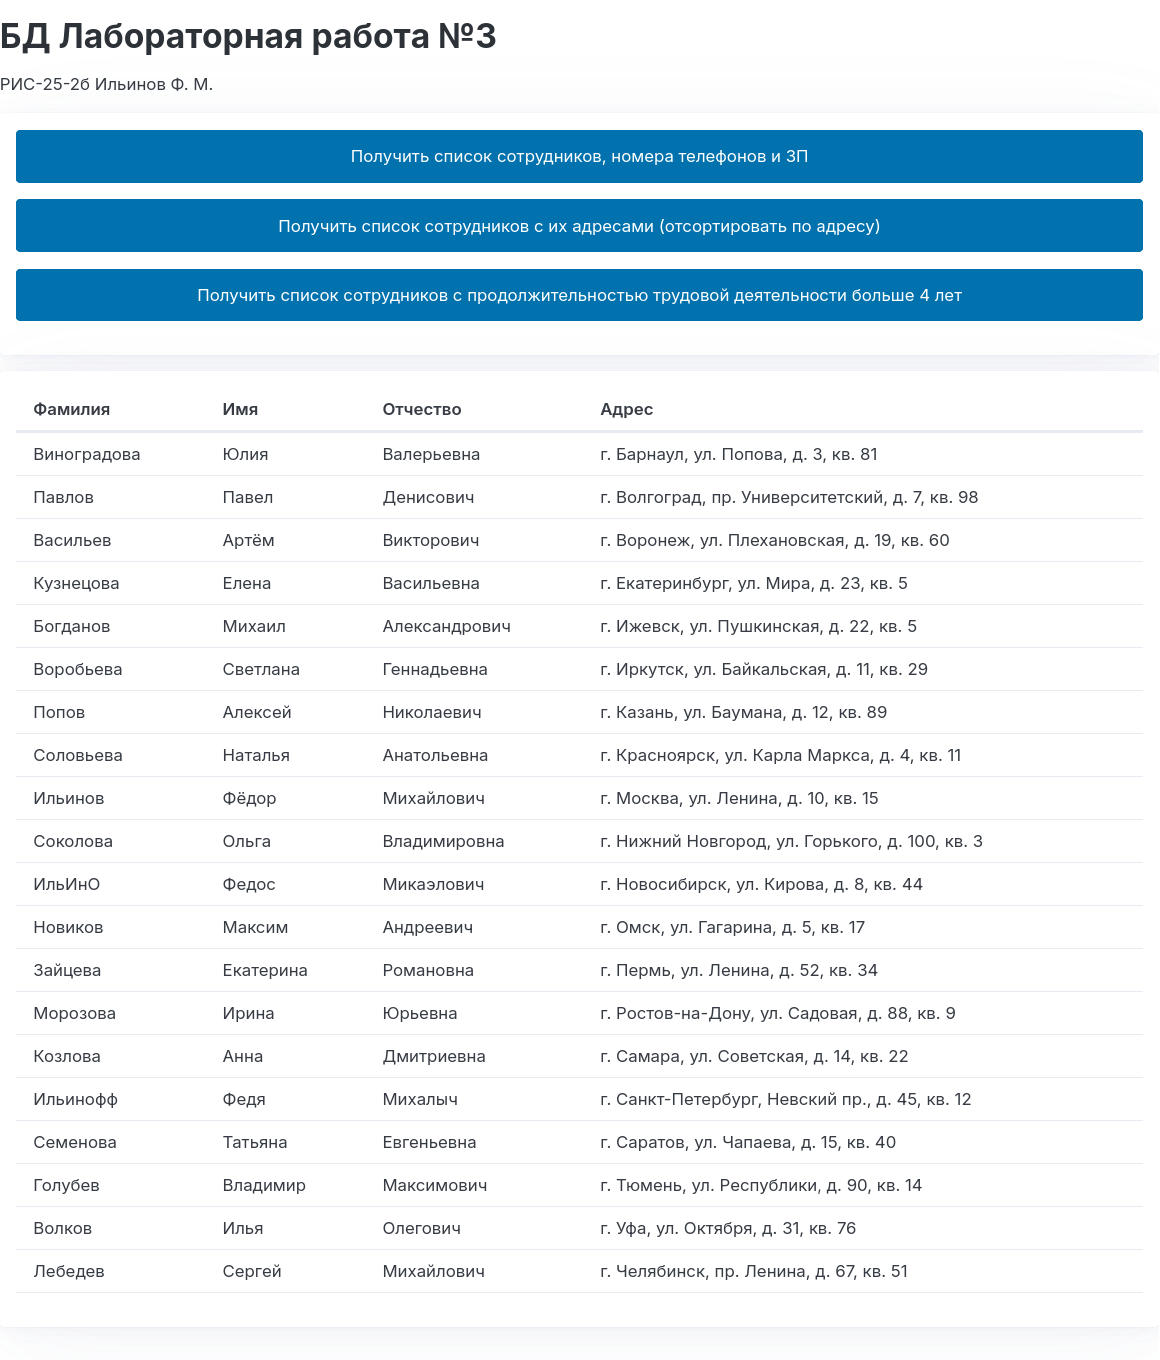
\includegraphics[width=1\textwidth]{img_query2_browser}
    \caption{Результаты выполнения второго запроса в браузере}
    \label{fig:fig-query2-browser}
\end{figure}

\begin{figure}[H]
    \centering
    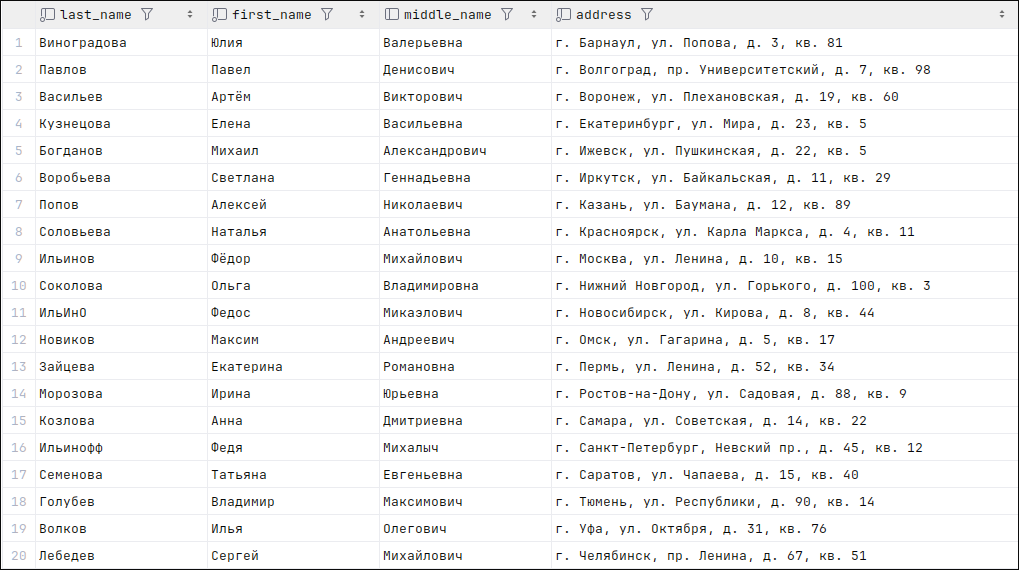
\includegraphics[width=1\textwidth]{img_query2_sql}
    \caption{Результаты выполнения второго запроса в просмотрщике баз данных}
    \label{fig:fig-query2-sql}
\end{figure}

Скриншот выполнения третьего запроса: список сотрудников с продолжительностью трудовой деятельности больше 4 лет
в браузере (рис. \ref{fig:fig-query3-browser}) и в просмотрщике баз данных (рис. \ref{fig:fig-query3-sql}).

\begin{figure}[H]
    \centering
    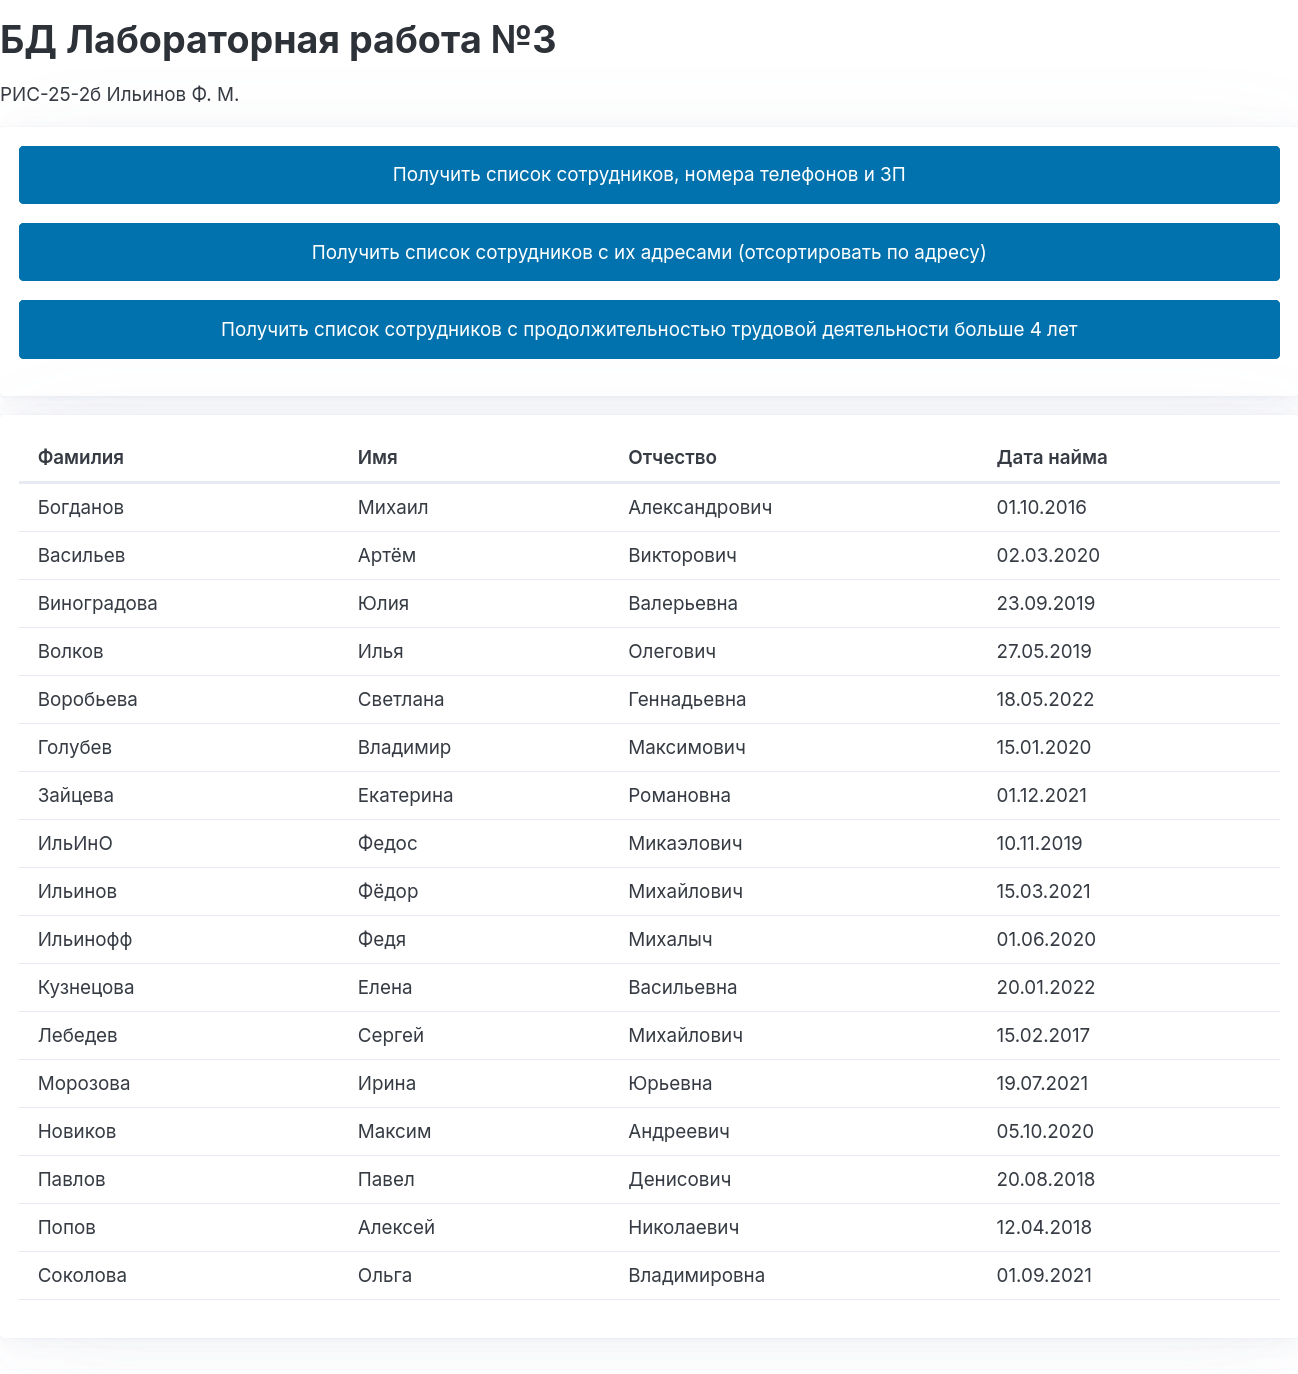
\includegraphics[width=1\textwidth]{img_query3_browser}
    \caption{Результаты выполнения третьего запроса в браузере}
    \label{fig:fig-query3-browser}
\end{figure}

\begin{figure}[H]
    \centering
    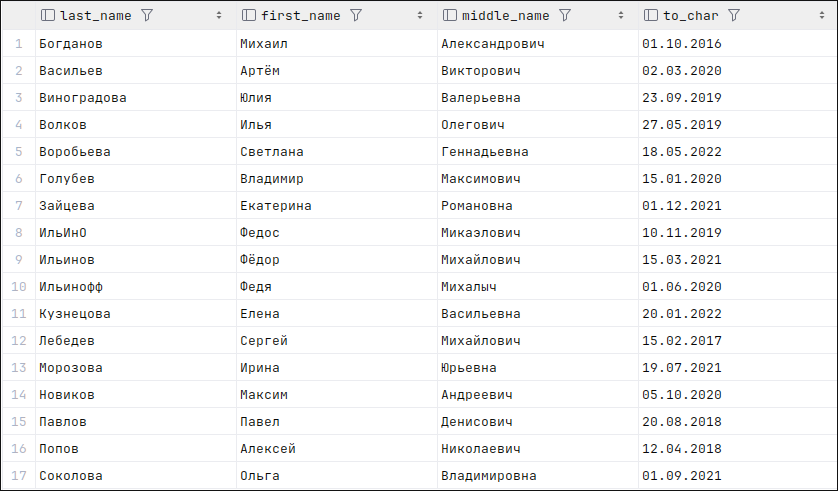
\includegraphics[width=1\textwidth]{img_query3_sql}
    \caption{Результаты выполнения третьего запроса в просмотрщике баз данных}
    \label{fig:fig-query3-sql}
\end{figure}

Как мы видим на приложенных рисунках, данные в браузере и в просмотрщике баз данных совпали.
Таким образом можно сделать вывод, что программа работает корректно.